
\begin{frame}
\section{}
Consider this model:

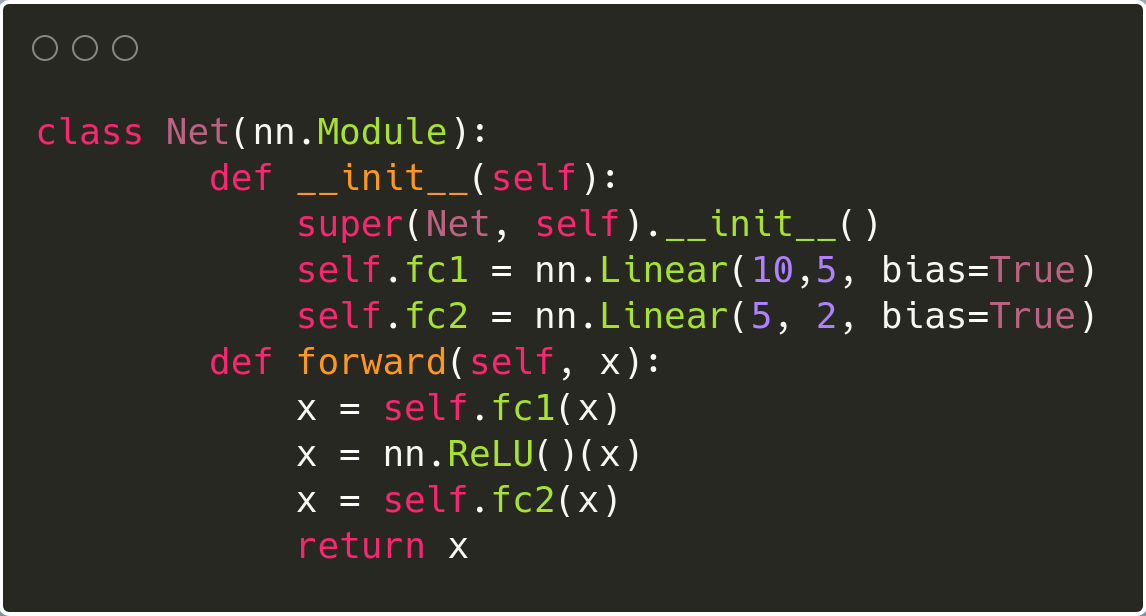
\includegraphics[width=0.7\textwidth]{images/quiz_4_4_2_1.png}

What is the number of trainable parameters in this model


\begin{enumerate}[label=(\Alph*)]
\item Depends on the input
\item 60
\item 62
\item 67    % Ans
\item None of these   % None
\end{enumerate}

\end{frame}


\begin{frame}
\section{}
Consider this model:

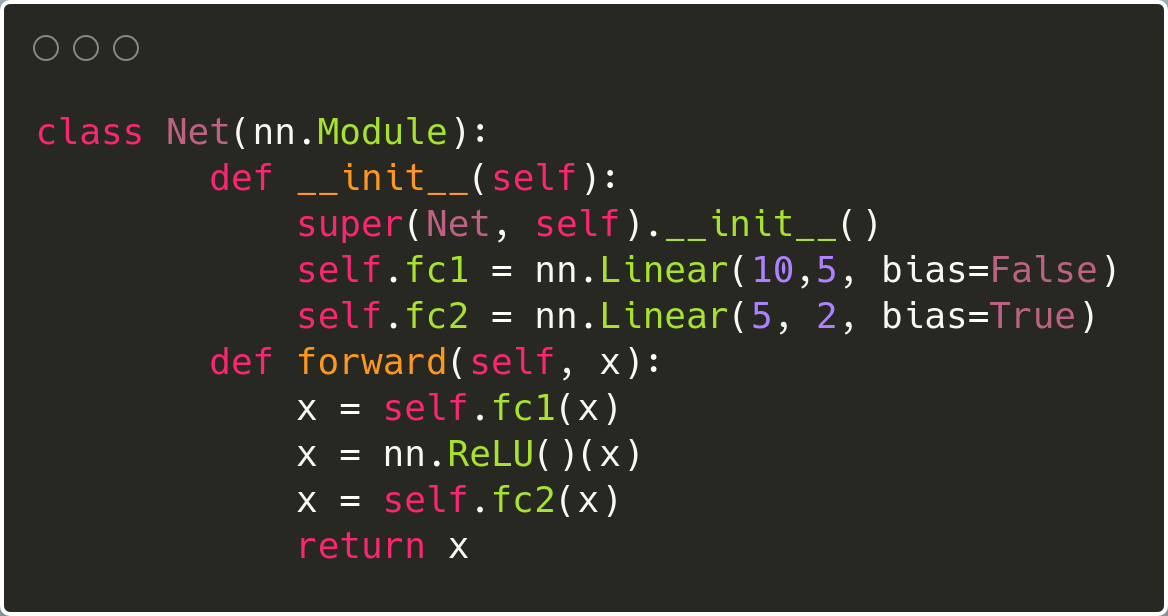
\includegraphics[width=0.7\textwidth]{images/quiz_4_4_2_2.png}

What is the number of trainable parameters in this model


\begin{enumerate}[label=(\Alph*)]
\item Depends on the input
\item 60
\item 62    % Ans
\item 67
\item None of these   % None
\end{enumerate}

\end{frame}


\begin{frame}
\section{}
Consider this model:

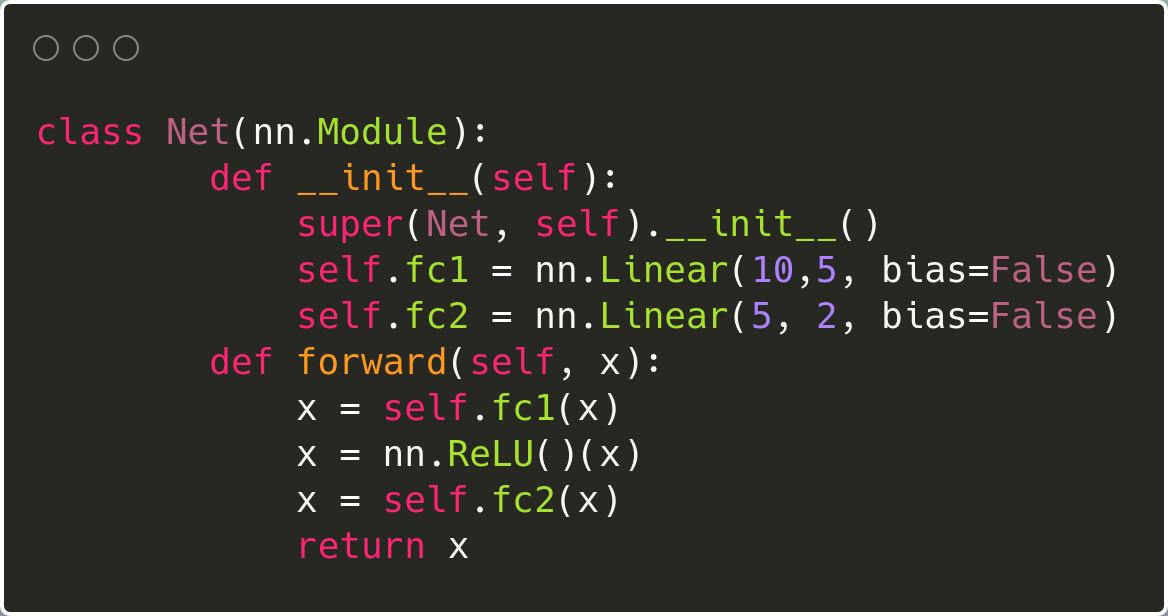
\includegraphics[width=0.7\textwidth]{images/quiz_4_4_2_3.png}

What is the number of trainable parameters in this model


\begin{enumerate}[label=(\Alph*)]
\item Depends on the input
\item 60    % Ans
\item 62
\item 67
\item None of these   % None
\end{enumerate}

\end{frame}


\begin{frame}
\section{}
Consider this model:

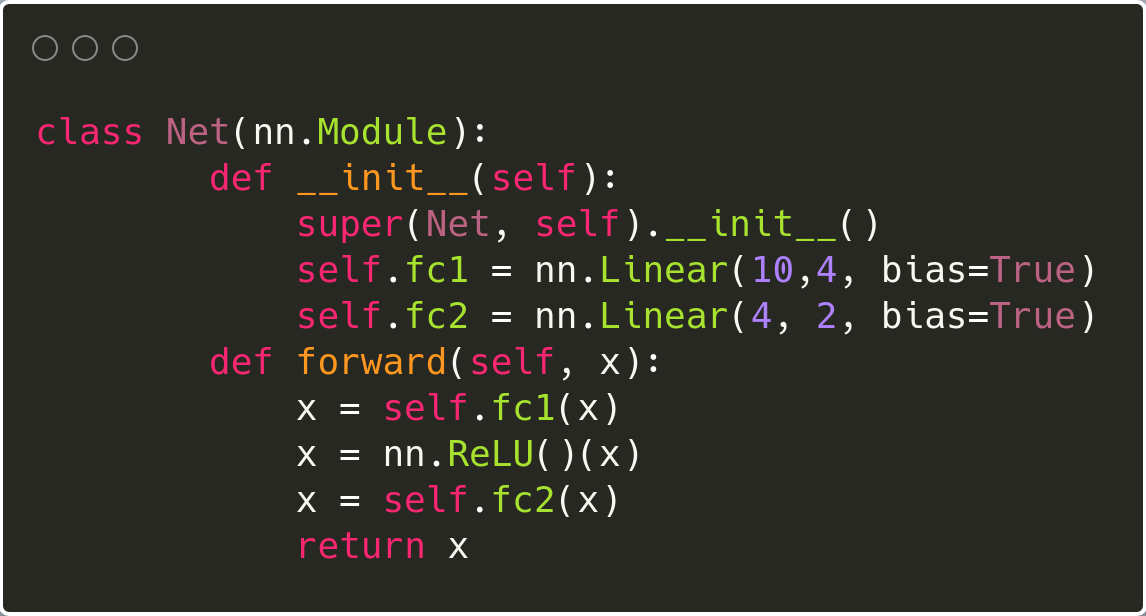
\includegraphics[width=0.7\textwidth]{images/quiz_4_4_2_4.png}

What is the number of trainable parameters in this model


\begin{enumerate}[label=(\Alph*)]
\item Depends on the input
\item 48
\item 50
\item 54     % Ans
\item None of these   % None
\end{enumerate}

\end{frame}


\begin{frame}
\section{}
Consider this model:

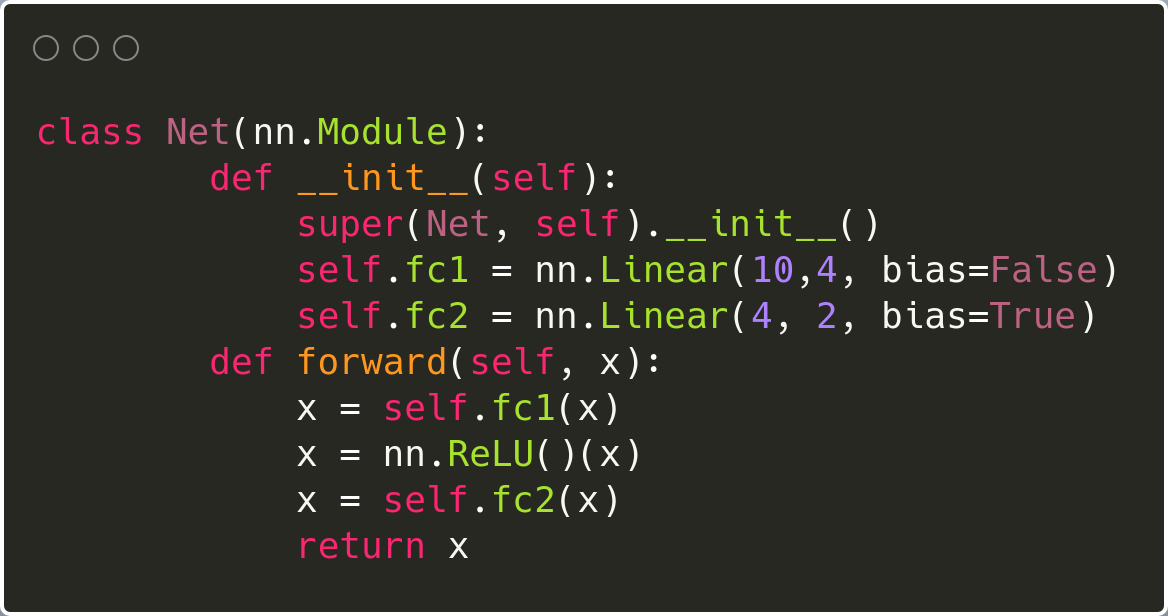
\includegraphics[width=0.7\textwidth]{images/quiz_4_4_2_5.png}

What is the number of trainable parameters in this model


\begin{enumerate}[label=(\Alph*)]
\item Depends on the input
\item 48
\item 50    % Ans
\item 54
\item None of these   % None
\end{enumerate}

\end{frame}


\begin{frame}
\section{}
Consider this model:

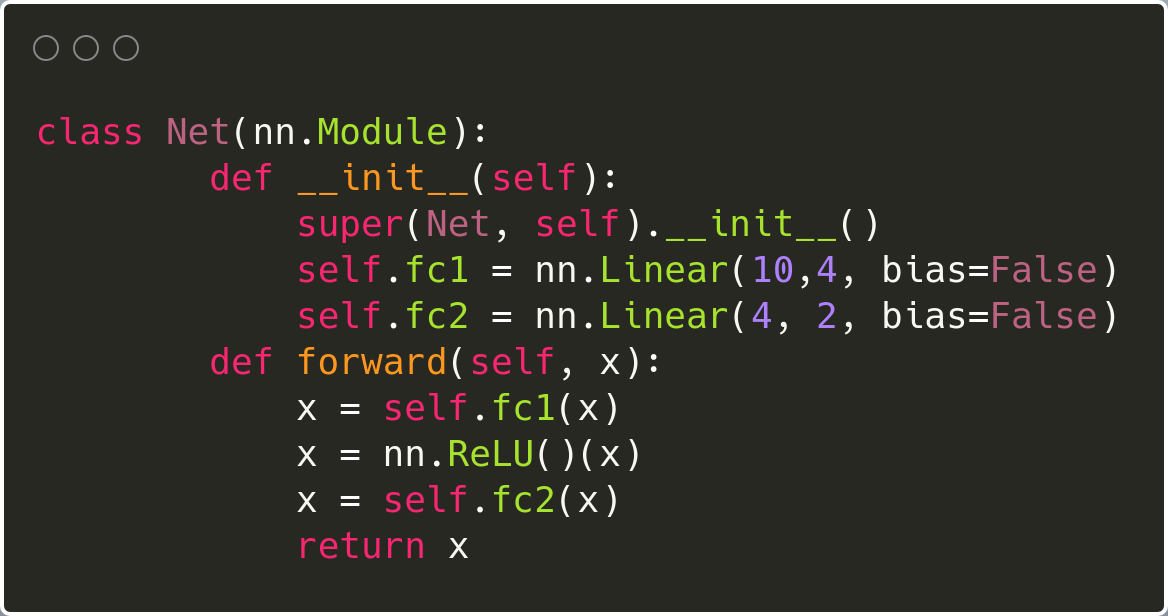
\includegraphics[width=0.7\textwidth]{images/quiz_4_4_2_6.png}

What is the number of trainable parameters in this model


\begin{enumerate}[label=(\Alph*)]
\item Depends on the input
\item 48    % Ans
\item 50
\item 54
\item None of these   % None
\end{enumerate}

\end{frame}
